\section{Evaluation}\label{sec:eval}

We ask five questions. \textbf{RQ2}: do existing tools find audited binding
flaws? \textbf{RQ3}: why does an LLM agent miss them, and what fixes it?
\textbf{RQ4}: do the gains hold on held-out data? \textbf{RQ5}: does \tool{}
find new flaws? \textbf{RQ6}: what do its warnings cost a human in precision,
evidence and time?

\subsection{Setup}\label{sec:eval-setup}

\para{Splits and versions}
We split the labeled findings by project family, never by item, with a fixed
seed, before anyone read test code. \tool{} was built in versions, each on
development data only and frozen before its test run. \emph{v2} (Stage~A)
was evaluated on the test families of benchmark B1. Because we then inspected
its misses, a dated amendment to our pre-registration moved the 13 B1
families into development before any later version ran on held-out data: 6
families (15 flaws) for tuning and 7 families (7 flaws, 3 hard negatives),
drawn with a seed, as a \emph{check set} that the building process never saw.
The final version, \emph{v4} (Stage~A, no-drop, multi-location and loop), was
built on \emph{dev-v4}: those 15 flaws plus the 13 original development flaws.
Appendix~\ref{app:timeline} lists who saw what, and when.

\para{Benchmarks}
All targets are cleaned snapshots without version history, audit text or
comments naming a finding.
\begin{itemize}
\item \textbf{B1, audited test set} (measures v2): 22 binding flaws in 13
families (15 in Solidity consumers, 2 in circuits, 5 in Rust guests or hosts),
14 \emph{hard negatives} (proof-related findings labeled not binding, at their
own locations) and 12 \emph{fixed twins} (the code after the fix). Round~2 (8
flaws) was located by a code-level pass whose results the building process
could not read.
\item \textbf{B2, mutants} (measures v2): 27 binding flaws injected into three
small hosts outside the dataset, at least four per pattern.
\item \textbf{Dev-v4} (builds v4): 28 flaws, 17 fixed twins and 28 hard
negatives in 41 snapshots; 18 Solidity, 3 circuit and 7 Rust flaws.
\item \textbf{Held-out} (measures v4): the \emph{check set}; \DEMO{\emph{round~3},
7 audited flaws from test families never used before, located after the
freeze}; and \emph{B3}, 37 mutants (11 on the proof side) in five open-source
applications outside every dataset family, with 5 decoys that stay bound and
the clean hosts as controls (Appendix~\ref{app:coverage}).
\end{itemize}

\para{Baselines}
Slither~\cite{slither} and Mythril~\cite{mythril} on build-enabled copies;
circomspect~\cite{circomspect} and Picus~\cite{picus}; Foundry invariant
fuzzing~\cite{foundry} out of the box and \emph{assisted}, with the binding
invariant of Section~\ref{sec:design-loop} wired by hand; and the same LLM as
a \emph{plain auditor} with a one-paragraph prompt and no ledgers.

\para{Scoring}
Matching rules were committed before each tool ran. A \emph{strict} hit names
the flaw's file and function and an LLM judge with a frozen prompt confirms
the mechanism; a \emph{loose} hit matches the location only; a
\emph{mechanism} hit reports the right mechanism anywhere. Related locations
are not credited, so a flaw reported on the other side of the seam scores
strictly only if that side is the auditor's. Judge verdicts are cached per
(warning, flaw) pair, so all configurations are judged identically; in a
re-judging test about one verdict in twenty flipped. A target a tool cannot
build is \emph{unsupported}, never a miss.

\para{Protocol}
LLM runs are stochastic. On dev-v4 every configuration ran twice per snapshot;
we report the \emph{union} (found in at least one run), the \emph{mean}, and
call a hit \emph{fragile} if it appears in one run only. Held-out numbers are,
as pre-registered, the \emph{median of three runs} with min--max, so dev and
held-out numbers are not directly comparable. Before the per-step
measurements we fixed a \textbf{keep rule}: a step is kept only if, against
the configuration it extends, (i) strict union recall gains at least 2, (ii)
it adds at most 1 new finding on fixed or hard-negative snapshots per 10 such
snapshots, and (iii) it yields no E2/E3 on them (Appendix~\ref{app:count}).
Intervals are Wilson 95\%~\cite{wilson1927}; paired comparisons use the exact
McNemar test~\cite{mcnemar1947}.

\subsection{RQ2: Existing tools on audited flaws}\label{sec:eval-rq2}

\begin{table*}[t]
\centering
\caption{Existing tools and \tool{} v2 on the audited test set B1 (strict
hits; 95\% Wilson interval). ``Analyzed'' counts round-1 flaws whose target
the tool could build and analyze; a flaw it could not is unsupported, not
missed. Specificity counts fixed twins and hard negatives without a warning
at the flaw's location.}
\label{tab:b1}
\footnotesize
\begin{tabular}{@{}lcccccc@{}}
\toprule
\textbf{Tool} & \textbf{Analyzed (R1)} & \textbf{Round 1 strict} & \textbf{of analyzed} & \textbf{Round 2 strict} & \textbf{Fixed spec.} & \textbf{HN spec.} \\
\midrule
Slither & 8/14 & 0/14 (0.00--0.22) & 0/8 & 0/8 (0.00--0.32) & 12/12 & 11/14 \\
Mythril & 8/14 & 0/14 (0.00--0.22) & 0/8 & \DEMO{0/8} & 6/6 & 6/6 \\
circomspect & 0/14 & unsupported & -- & \DEMO{unsupported} & 6/6 & 5/6 \\
Picus & 0/14 & unsupported & -- & unsupported & -- & -- \\
Foundry, out of box$^\dagger$ & 11/14 & \multicolumn{3}{c}{0/13 analyzed (R1+R2)} & -- & -- \\
Foundry, assisted$^\dagger$ & 11/14 & \multicolumn{3}{c}{5/13 analyzed (0.18--0.64)} & 2/4$^\ddagger$ & 3/3 \\
Plain LLM, 1 run & 14/14 & 3/14 (0.08--0.48) & 3/14 & -- & 6/6 & 6/6 \\
\tool{} v2, 1 run & 14/14 & 4/14 (0.12--0.55) & 4/14 & 2/8 (0.07--0.59) & 12/12 & 12/14 \\
\quad mechanism level & & 5/14 & & 4/8 & & \\
\bottomrule
\multicolumn{7}{@{}p{0.95\textwidth}}{\scriptsize $^\dagger$Covers the 13 EVM-side flaws of both rounds; circuit- and guest-side flaws are unsupported. Harnesses were wired by hand in 5--45 min per target; a fuzzer hit is a property violation at the labeled mechanism. $^\ddagger$Two fixed twins flagged: in one the fix is not visible at the level the harness exercises, in the other it changed which configuration is trusted.}
\end{tabular}
\end{table*}

Table~\ref{tab:b1} shows the result on real audited flaws. Neither Solidity
analyzer reports any flaw at the right location and mechanism; Slither and
Mythril report \emph{something} at the location of 3 and 2 flaws, but none
describes the binding mechanism. The circuit analyzers fail for a different
reason: most flaws are not in a circuit. Out of the box, the fuzzer finds none
of the 13 flaws it can run on despite up to millions of calls per target,
because a binding flaw crashes nothing; the contract works exactly as
written.

\para{The missing piece is the specification}
Given the binding invariant---an honest proof resubmitted by a second account
with changed arguments must not produce a different effect---the same
fuzzer finds 5 of the 13 and raises no alarm on 3 hard negatives. The
difference between 0 and 5 is entirely the specification, which took 5--45
minutes of expert wiring per target and cannot express circuit- or
guest-side flaws. \tool{} v2 infers it: on the same 13 EVM-side flaws it
finds 6 strictly with no human setup. The two overlap on 3; 3 are found only
by v2 and 2 only by the fuzzer.

\para{An LLM agent is better, but not good}
v2 finds 6 of the 22 audited flaws strictly (9 at mechanism level), with no
strict warning on 12 fixed twins. On the 27 B2 mutants it finds 22, including
all 4 circuit-side ones (Appendix~\ref{app:extra}). The gap to the analyzers is
categorical, but the gap to the plain LLM is small (4 vs.\ 3 of 14 on round
1), all six strict hits are in Solidity consumers, and v2 finds none of the 7
circuit or Rust flaws of B1.

\finding{Analyzers find no binding flaw and a fuzzer finds them only when a
human supplies the binding specification. An LLM agent infers that
specification, but on real audited code it still misses most flaws, all
proof-side ones included.}

\subsection{RQ3: Why the agent misses, and what fixes it}\label{sec:eval-anatomy}

\para{First diagnosis: judgment, not reading}
We traced every miss of a v2 run set on the 28 dev-v4 flaws through the scan
transcripts. In every case the flawed code reached the agent; no miss was
caused by not reading. The misses were verdicts (judged bound, unknown, or
found and withdrawn), reports at the other end of the binding, and three
questions never asked (a chain ID missing from a signed message, a parser
differential, an unanchored library getter). Twelve concern what the proof
side commits. This suggested two remedies, more knowledge and a second look,
and a third we had not planned: stop the agent from discarding what it
already wrote down. We built all of them as separate steps
(Section~\ref{sec:design}) and measured each under the keep rule.

\begin{table}[t]
\centering
\caption{Configurations on dev-v4 (28 flaws, 41 snapshots, 2 runs each;
measured). $\cup$/$\mu$: union/mean over runs. Fix: fixed twins flagged at
strict/loose. New/10: new findings on the 29 fixed or hard-negative snapshots
per 10, relative to the configuration extended (two v2 runs differ by 1.72).
F/s: findings per snapshot. \$: median per scan.}
\label{tab:dev}
\footnotesize
\setlength{\tabcolsep}{2.6pt}
\resizebox{\columnwidth}{!}{%
\begin{tabular}{@{}lrrrrcrrr@{}}
\toprule
\textbf{Configuration} & \textbf{S$\cup$} & \textbf{S$\mu$} & \textbf{L$\cup$} & \textbf{M$\cup$} & \textbf{Fix} & \textbf{New/10} & \textbf{F/s} & \textbf{\$} \\
\midrule
v2 (Stage A) & 12 & 10.0 & 15 & 17 & 0/1 & (1.72) & 1.5 & 0.84 \\
\quad + no-drop only & 17 & 13.0 & 19 & 20 & 0/3 & 2.76 & 2.4 & 0.90 \\
\rowcolor{blue!6}\textbf{v4: + no-drop + multi-loc.} & \textbf{18} & \textbf{14.0} & 20 & 20 & 0/4 & \textbf{0.52} & 1.7 & 0.99 \\
\midrule
\multicolumn{9}{@{}l}{\emph{extensions, relative to v4 (rejected)}} \\
\quad + challenge & 20 & -- & -- & -- & -- & 1.90 & -- & \\
\quad + inventory & 18 & -- & -- & -- & -- & 1.72 & -- & \\
\quad + probes & 19 & -- & -- & -- & -- & 4.48 & -- & \\
\quad + knowledge & 18 & 16.5 & 21 & 20 & -- & 3.45 & -- & \\
\multicolumn{9}{@{}l}{\emph{relative to v2 (rejected)}} \\
\quad Stage A + knowledge & 16 & 15.0 & 18 & 20 & -- & 3.97 & -- & \\
\quad all post steps & 20 & 17.5 & 23 & 23 & 1/7 & 7.93 & 3.2 & 1.62 \\
\bottomrule
\end{tabular}}
\end{table}

\para{Keeping what the agent found}
Table~\ref{tab:dev} gives the result. With identical model, runs and judge,
v4 finds 18 of 28 flaws strictly over two runs (64\%, 95\% CI 46--79\%)
against 12 for v2 (43\%, 27--61\%); per run, 14.0 against 10.0. The
comparison is paired over the same Stage~A runs, so v4 cannot lose a v2 hit
by construction (additivity); 6 flaws are gained (exact McNemar $p=0.031$).
No fixed twin is flagged at strict (0 of 17). The cost is visible elsewhere:
hard negatives flagged rise from 2 to 4 of 28, fixed twins matched at
location only from 1 to 4 (the judge rejects the mechanism in every case),
and raw warnings per snapshot double (1.5 to 3.1) while findings rise only
from 1.5 to 1.7. No-drop alone recovers 5 flaws but, counting each restored
warning as a new finding, adds 2.76 per 10 on fixed and hard-negative
snapshots and fails the rule; multi-location grouping attaches most restored
warnings to the finding they belong to and brings the pair to 0.52, inside
run-to-run noise. Part (iii) of the rule could not be measured during the
build: the loop's scaffold failed to compile against recent libraries
(Section~\ref{sec:eval-rq6}). The
post-stage costs a median \$0.15 and 29\,s per scan and never reads the
repository. Loose recall rises from 15 to 20 and mechanism recall from 17 to
20, so about half of the strict gain is \emph{placement}: the right
mechanism moved to the auditor's side of the seam.

\begin{figure}[t]
\centering
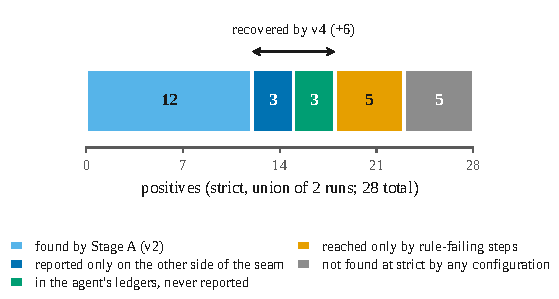
\includegraphics[width=\columnwidth]{fig-loss.pdf}
\caption{Anatomy of strict recall on dev-v4 (union of 2 runs, measured).
Each recovered hit is traced to the judge-accepted warning and the no-drop
candidate or multi-location sibling that produced it. ``v4 kept'' denotes v4.}
\label{fig:loss}
\end{figure}

\para{Anatomy of the gain}
Figure~\ref{fig:loss} partitions the 28 flaws. Stage~A finds 12. Each of the
6 recovered flaws was already in the agent's working state. \emph{Placement
(3)}: Stage~A reported the root cause, but on the other side of the seam; the
hit comes from a row no-drop restored at the auditor's location or from a
multi-location sibling. \emph{Never reported (3)}: the value sat in an
unbound row, an unconstrained statement row or a withdrawn draft, dismissed
once because the consuming contract ``is not in the repository'' and once
because the value at stake seemed too small. Across all 82 Stage~A runs the agent left
427 recorded suspicions without a final warning of their own (239 unbound
effect rows, 146 unconstrained statement rows, 42 withdrawn drafts), about 5
per run. No-drop found an admissible reason to drop 317. It restored 110,
merged into 72 warnings, 0.9 per run; by keyword coding of its stated
reasons, roughly 80 had been reported only at another location and 30 not at
all.

\para{Case study: a zkVM light client}
A light-client contract accepts a zkVM receipt and stores new headers, state
roots and the next sync committee. The guest reads the whole starting store
from private input and commits only a hash of the starting committee.
Stage~A's statement ledger recorded \emph{prevHeader: constrained: no; read
from program input, never compared to a public input}, yet its final answer
reported the problem only at the contract's \texttt{update}; the auditor
located it in the guest. No-drop dropped six candidates as covered and two
as harmless, but restored three statement rows, because their primary
location, the guest's \texttt{main}, differs from the warning's.
Multi-location then linked guest and contract under one finding. The item
went from 0 to 2 strict hits, both from tool-less calls.

\para{More knowledge, more looking, less specificity}
Three of the four extensions raised recall, and all four failed the rule
(Table~\ref{tab:dev}, Figure~\ref{fig:tradeoff}). \emph{Knowledge} alone
raises strict recall from 12 to 16 and makes hits more stable (mean 15.0),
but on top of v4 the union stays at 18: it finds earlier what no-drop
recovers later, and it adds Stage~A findings on patched and hard-negative
code well above run-to-run noise. \emph{Challenge} buys two flaws for about
5.5 new findings per run on those snapshots, \emph{probes} one for 13, and
\emph{inventory} none. These findings recur in both runs on the same
snapshots, so they reflect what the steps look for, not noise; whether some
are real issues outside the label set we cannot say without triage, so the
rule counts them all. A catalogue teaches the agent to \emph{suspect} more;
no-drop stops it \emph{losing} what it already suspects, which is cheaper and
far more specific. Pursuing recall without the rule would have reached 20 of
28 at 7.93 new findings per 10 and twice the volume.

\begin{figure}[t]
\centering
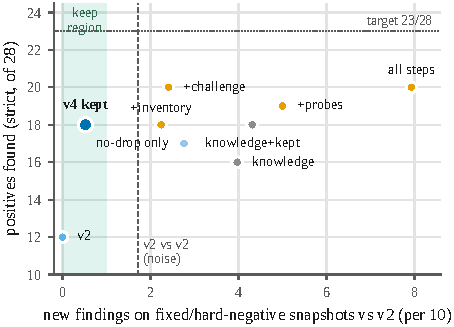
\includegraphics[width=\columnwidth]{fig-tradeoff.pdf}
\caption{Strict recall against new findings on fixed and hard-negative
snapshots, relative to v2 (dev-v4, measured). The shaded band is the keep
rule's tolerance; the dashed line is v2 against itself. Only v4 lies inside
the band. The dotted line is the 80\% target set before the build. ``v4 kept'' denotes v4.}
\label{fig:tradeoff}
\end{figure}

\begin{table}[t]
\centering
\caption{Strict union recall on dev-v4 by pattern (measured).}
\label{tab:pattern}
\footnotesize
\begin{tabular}{@{}lrrrr@{}}
\toprule
\textbf{Pattern} & \textbf{Flaws} & \textbf{v2} & \textbf{v4} & \textbf{All steps} \\
\midrule
P1 effect & 8 & 5 & 7 & 7 \\
P2 context & 10 & 4 & 6 & 8 \\
P3 replay & 3 & 2 & 3 & 2 \\
P4 verifier & 3 & 1 & 2 & 2 \\
P5 interface & 3 & 0 & 0 & 1 \\
other & 1 & 0 & 0 & 0 \\
\bottomrule
\end{tabular}
\end{table}

\para{What remains}
Five flaws are found by no configuration: a parser differential between the
signed and the parsed region of an e-mail, a library getter that skips its
sibling's anchor check, a chain identifier that stays a prover input, a
verifier chosen from a class anyone can register, and a batch check that does
not tie each (image, journal) claim to its request. Each requires following
the value into a library, a registry or an aggregation helper that the
consumer function does not show. Five more are reached only by rejected
steps. By pattern (Table~\ref{tab:pattern}), gains concentrate in P1 and P2;
interface mismatches (P5) remain unsolved, 0 of 3. Stability is also a limit (Figure~\ref{fig:items}): 8 of v4's 18 hits are
fragile, so a single run finds about 14 and a second adds about 4
(Appendix~\ref{app:items}). Knowledge makes hits more stable (3 fragile)
but not broader.

\begin{figure*}[t]
\centering
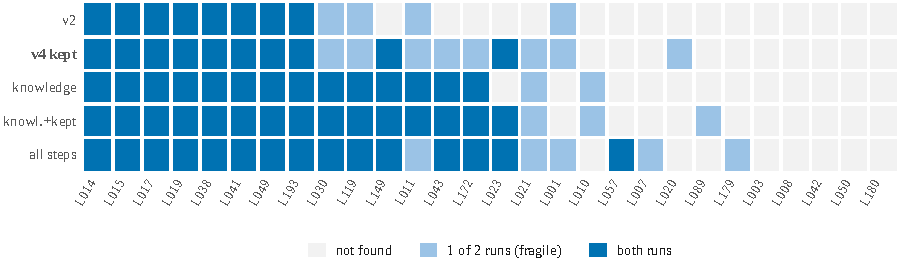
\includegraphics[width=\textwidth]{fig-items.pdf}
\caption{Strict outcome per dev-v4 flaw (columns) and configuration (rows) over
two runs, sorted by total hits (measured). ``v4 kept'' denotes v4.}
\label{fig:items}
\end{figure*}

\finding{The agent's recoverable misses were not unseen: it reported them on
the wrong side of the proof boundary or recorded them and let them go. One
tool-less re-adjudication under closed rules recovers them (12$\to$18 of
28 over two runs, 10.0$\to$14.0 per run, $p=0.031$) with no strict false finding on patched code, while knowledge
and extra tool-using looks buy recall only with false findings.}

\subsection{RQ4: Held-out data}\label{sec:eval-heldout}

\begin{table}[t]
\centering
\caption{\DEMO{Frozen v4 on held-out data: strict hits, median of three runs
(min--max).} v2's single pre-amendment run on the check set found 2 of 7
(measured). Fresh audited = check set + round~3.}
\label{tab:final}
\footnotesize
\setlength{\tabcolsep}{3pt}
\begin{tabular}{@{}lccc@{}}
\toprule
\textbf{Set (positives)} & \textbf{v2} & \textbf{Plain LLM} & \textbf{v4} \\
\midrule
Check set (7) & \DEMO{2 (2--3)} & \DEMO{2 (1--2)} & \DEMO{3 (3--4)} \\
Round~3 (7) & \DEMO{2 (1--2)} & \DEMO{1 (1--2)} & \DEMO{3 (2--4)} \\
\textbf{Fresh audited (14)} & \DEMO{4 (3--5)} & \DEMO{3 (2--4)} & \DEMO{\textbf{6} (5--7)} \\
\quad union of 3 runs & \DEMO{5} & \DEMO{4} & \DEMO{8} \\
\quad mechanism level & \DEMO{6} & \DEMO{5} & \DEMO{8} \\
B3 mutants (37) & \DEMO{21 (20--23)} & \DEMO{11 (9--12)} & \DEMO{\textbf{27} (25--29)} \\
\quad proof side (11) & \DEMO{3} & \DEMO{1} & \DEMO{6} \\
\midrule
Decoys flagged (5) & \DEMO{0} & \DEMO{2} & \DEMO{1} \\
Hard negatives flagged (3) & \DEMO{0} & \DEMO{0} & \DEMO{1} \\
\bottomrule
\end{tabular}
\end{table}

\DEMO{v4 was frozen, and its tag and file hashes appended to the
pre-registration, before it ran on any held-out set. On the 14 fresh audited
flaws it finds a median of 6 (43\%, 95\% CI 21--67\%) against 4 for v2 and 3
for the plain LLM (Table~\ref{tab:final}); over three runs it finds 8. On B3
it finds 27 of 37 mutants (73\%) against 21 and 11, and 6 of the 11
proof-side ones against 3. v2 and v4 ran independently, so v4 can lose hits;
counting a flaw as found when a tool finds it in at least two of its three
runs, v4 gains 10 and loses 2 against v2 over all 51 held-out flaws (exact
McNemar $p=0.04$); 8 of the 10 gains come from
restored or sibling warnings, the same mechanism as on dev. It flags one of
five decoys and one of three hard negatives, and no fixed twin at strict.
The held-out gain is smaller than the dev gain, as expected for a method
developed on dev data; the held-out audited recall (43\%) is below the
single-run dev recall (50\%).}

\begin{figure}[t]
\centering
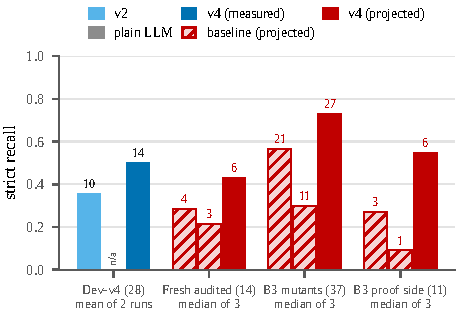
\includegraphics[width=\columnwidth]{fig-heldout.pdf}
\caption{Strict recall on dev-v4 (measured, mean of 2 runs) and on held-out
sets (\DEMO{projected, median of 3 runs}). The plain LLM was not run on
dev-v4.}
\label{fig:heldout}
\end{figure}

\finding{\DEMO{The improvement transfers: on 51 held-out flaws, v4 gains 10
and loses 2 against v2, mostly through the same placement and
non-reporting repairs. Proof-side flaws remain the hardest: v4 finds about
half.}}

\subsection{RQ5: New binding flaws}\label{sec:eval-rq5}

\DEMO{We ran frozen v4 once, as pre-registered, on the latest audited
commits of 25 ZK applications from our collection that were never used in
development or evaluation. It reported 46 findings (1.8 per application). Two
authors judged each independently from its evidence (phase~2,
Section~\ref{sec:eval-rq6}): 9 are binding flaws, of which 6 match findings
the auditors had already reported and 3 are previously unreported
(Table~\ref{tab:new}). We confirmed each new flaw with an attack test that a
second author re-ran, checked whether the current release is affected, and
reported it through the project's security contact. In N1, a
social-recovery module accepts a proof over an account's guardians but takes
the new owner set from calldata, so anyone who observes a valid recovery
proof can install its own owners.}

\begin{table}[t]
\centering
\caption{\DEMO{Previously unreported binding flaws found by \tool{}.} Evid.:
strongest executed evidence (E3 real proof, E2 mock verifier). Projects are
anonymized until disclosure completes.}
\label{tab:new}
\footnotesize
\setlength{\tabcolsep}{2.5pt}
\begin{tabular}{@{}llllll@{}}
\toprule
\textbf{ID} & \textbf{Domain} & \textbf{Pat.} & \textbf{Unbound value} & \textbf{Evid.} & \textbf{Status} \\
\midrule
\DEMO{N1} & \DEMO{social recovery} & \DEMO{P1} & \DEMO{new owner set} & \DEMO{E3} & \DEMO{fixed} \\
\DEMO{N2} & \DEMO{bridge} & \DEMO{P2} & \DEMO{source chain ID} & \DEMO{E3} & \DEMO{acknowledged} \\
\DEMO{N3} & \DEMO{token claim} & \DEMO{P3} & \DEMO{nullifier mod $r$} & \DEMO{E2} & \DEMO{no reply (40\,d)} \\
\bottomrule
\end{tabular}
\end{table}

\subsection{RQ6: Precision, evidence and cost}\label{sec:eval-rq6}

\para{Two-phase ground truth}
Audit labels bound recall but not precision: a finding that matches no label
is either false or a flaw the auditor missed. Phase~1 matches findings to
labels or mutants; phase~2 sends every unmatched finding to two authors, who
judge it independently from its evidence package with C1--C3 as the rubric,
then resolve disagreements. \DEMO{They agreed on 86\% of the 113 phase-2
findings before discussion ($\kappa=0.74$).}

\begin{table}[t]
\centering
\caption{\DEMO{Every v4 finding on the blind sets.} Corr.: matched a label or
mutant, or (hunt) judged a real binding flaw in phase~2; Pol.: real but allowed by $\Pi$; Unc.:
undecided; Test: correct / false findings with a succeeding attack test (E2
or E3); Min: median review minutes per project.}
\label{tab:evidence}
\scriptsize
\setlength{\tabcolsep}{2.4pt}
\begin{tabular}{@{}lrrrrrrrr@{}}
\toprule
\textbf{Set} & \textbf{Find.} & \textbf{Corr.} & \textbf{Pol.} & \textbf{Unc.} & \textbf{FP} & \textbf{Prec.} & \textbf{Test} & \textbf{Min} \\
\midrule
Check + round 3 & \DEMO{26} & \DEMO{6} & \DEMO{6} & \DEMO{4} & \DEMO{10} & \DEMO{23\%} & \DEMO{3 / 1} & \DEMO{14} \\
B3 mutants & \DEMO{74} & \DEMO{27} & \DEMO{9} & \DEMO{7} & \DEMO{31} & \DEMO{36\%} & \DEMO{18 / 2} & \DEMO{7} \\
Hunt & \DEMO{46} & \DEMO{9} & \DEMO{7} & \DEMO{5} & \DEMO{25} & \DEMO{20\%} & \DEMO{6 / 1} & \DEMO{24} \\
\midrule
Total & \DEMO{146} & \DEMO{42} & \DEMO{22} & \DEMO{16} & \DEMO{66} & \DEMO{29\%} & \DEMO{27 / 4} & \\
\bottomrule
\end{tabular}
\end{table}

\para{Precision}
\DEMO{Of v4's 146 findings on the blind sets, 42 are correct (29\%, 95\% CI
22--37\%) and 22 more describe real caller-chosen values that the intended
policy allows (Table~\ref{tab:evidence}); phase~2 found no unlabeled binding
flaw on the audited or mutant sets. Precision depends on the target: 36\% on
mutants, 23\% on audited code and 20\% in the hunt, where the code has
already passed an audit and most findings concern paths the audit covered.
An auditor reads about two findings per project, each with its proof-side and
consumer-side locations.}

\para{Executable evidence}
\DEMO{After we made the scaffold derive its EVM version from the sources (a
fixed target had failed on a vendored library that uses a newer opcode), 7 of
v4's 18 dev hits reached E2 and 3 reached E3, with no E2 or E3 on the 29
fixed or hard-negative snapshots, which satisfies part (iii) of the keep
rule. On the blind sets, 27 of the 42 correct findings carry a succeeding
test, against 4 of the 66 false ones. A finding with a passing test took a
median of 6 minutes to review, one without 15 (6 against 11 within B3, where
mutants are alike); this is an association, not a controlled effect.}

\para{Cost}
On dev-v4, Stage~A takes a median of 244\,s (76--615\,s) and \$0.84
(\$0.19--2.90) per scan, scaling with repository size
(Appendix~\ref{app:extra}); the post-stage adds 29\,s and \$0.15. The loop
adds a median of \$0.39 (at most \$2.40) on development targets, 80\% of it
for drafting scaffolds; template attempts cost nothing. \DEMO{On the
held-out sets a full scan costs a median of \$1.46 and 6.2 minutes.} The
analyzers run in minutes but only after a human has made each project build,
and the assisted fuzzer needs 5--45 minutes of expert wiring per target.

\finding{\DEMO{About three findings in ten are real binding flaws and two
more in ten are policy-allowed; a passing attack test separates them well
(27 of 42 correct, 4 of 66 false). A scan costs about \$1.50.}}
